\section{Visualization of Multi-Turn Agent-User Dialogs and Generated Images}
In \Cref{fig:dialog}, we show examples of multi-turn dialogs between simulated users and the three agents in \Cref{sec:exp}. We also visualize the generated images in \Cref{fig:toy1}, \Cref{fig:toy2}, \Cref{fig:coco1} and \Cref{fig:coco2}.
\begin{figure}
    \centering
    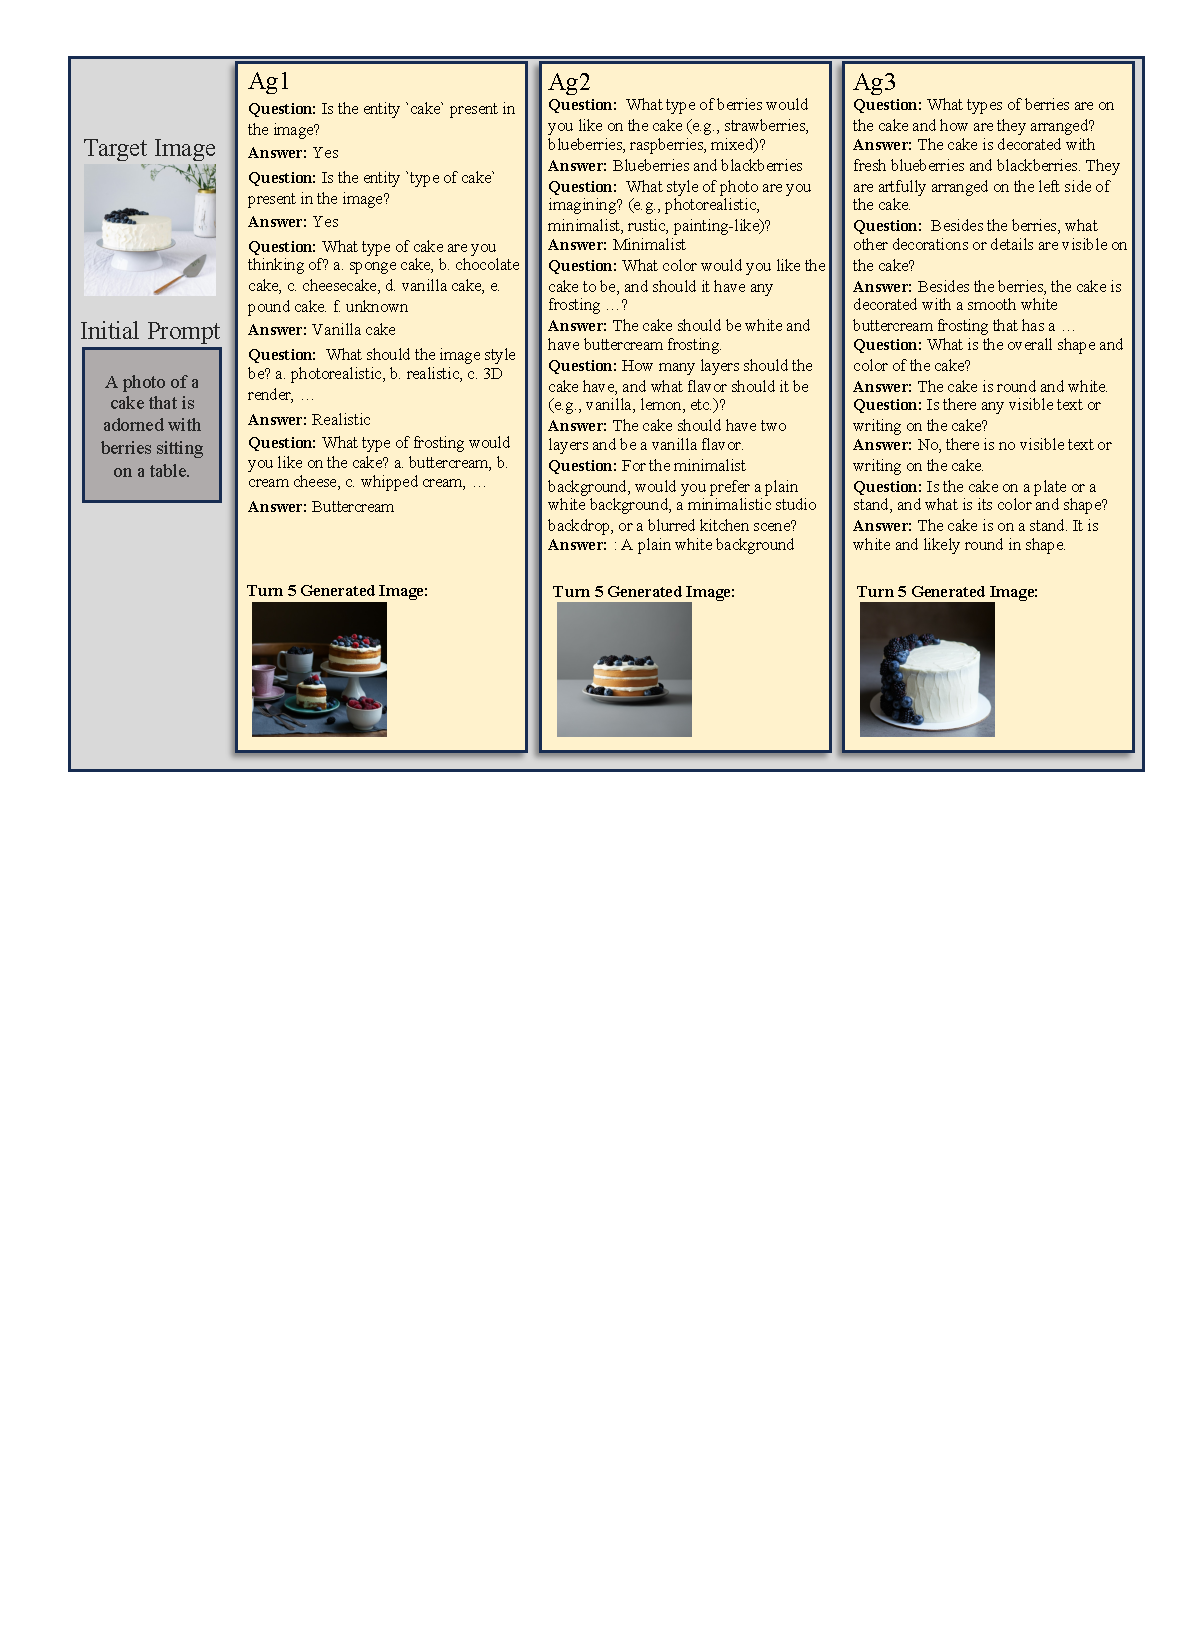
\includegraphics[width=\linewidth]{figures/dialog.pdf}
    \caption{Real multi-turn dialogs generated by the Ag1, Ag2, and Ag3 agents on an image from DesignBench. The figure additionally shows the image generated after the 5 turn dialog per agent.}
    \label{fig:dialog}
\end{figure}

\begin{figure}
    \centering
    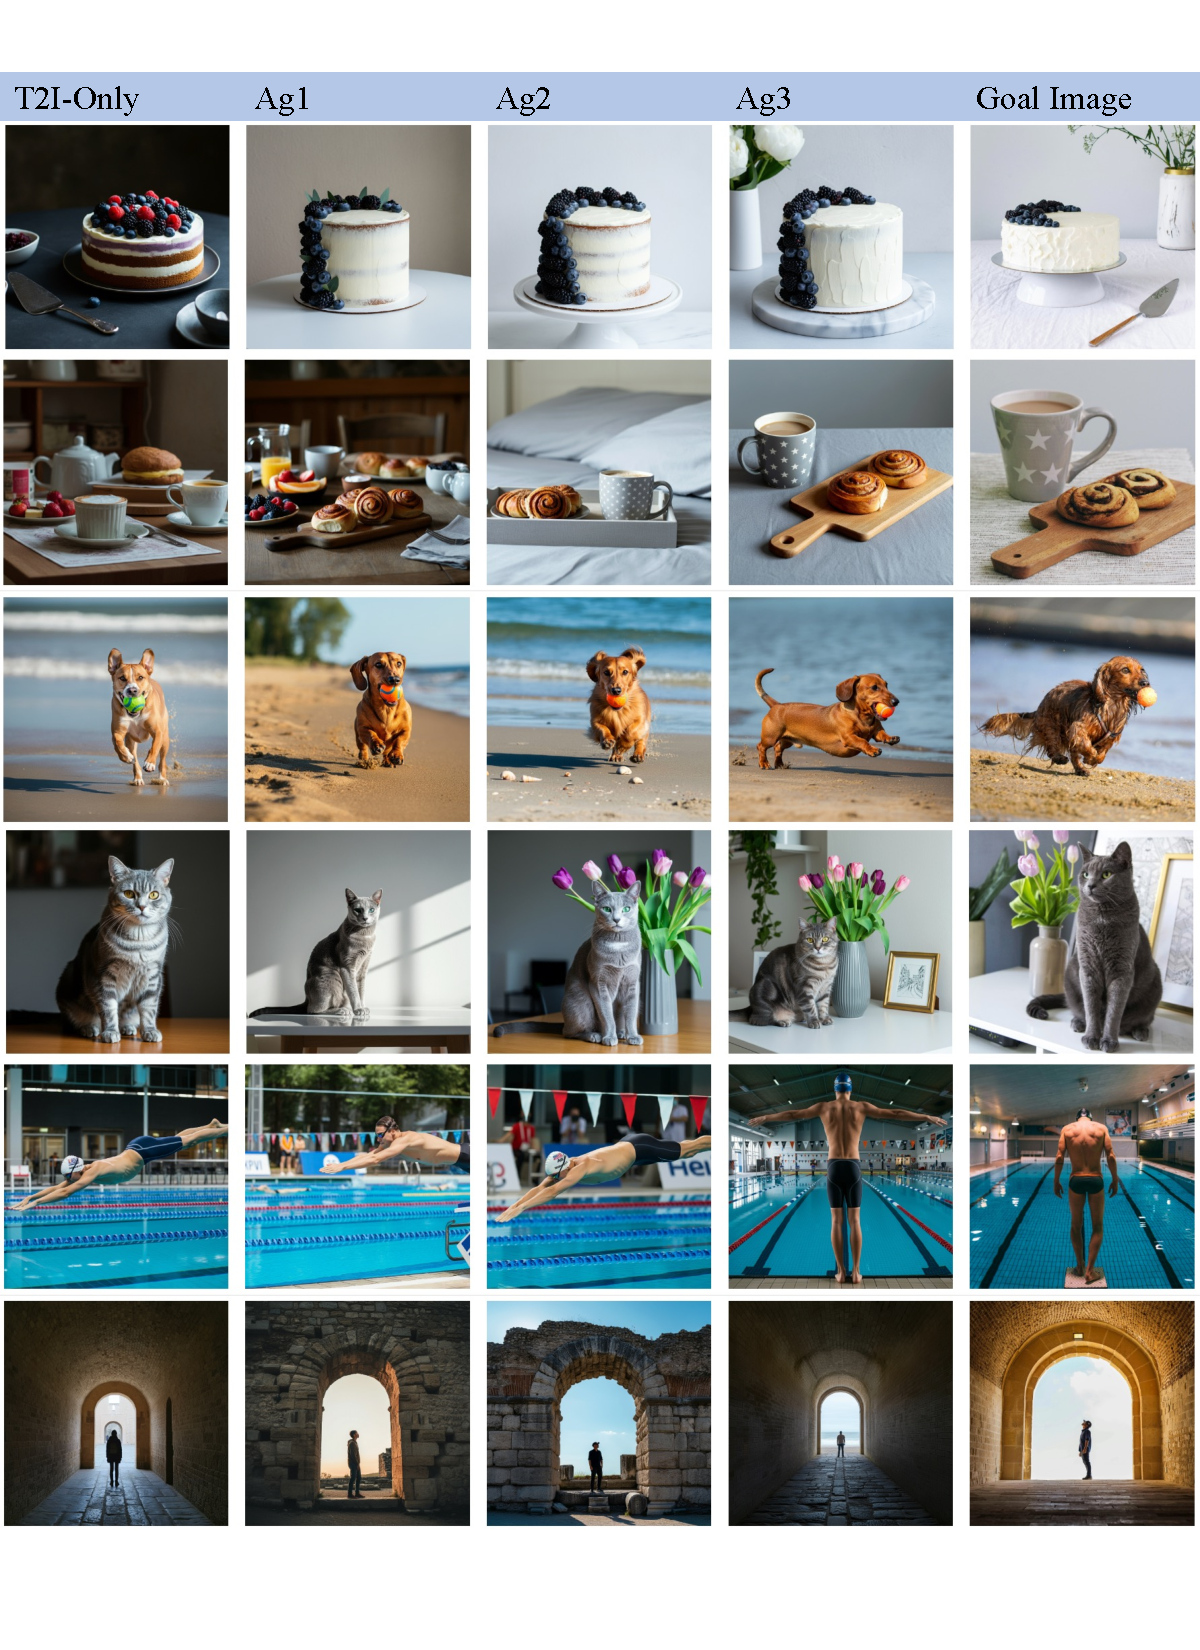
\includegraphics[width=\linewidth]{figures/toy_data_chart_part1.pdf}
    \caption{Agent Generated Image Outputs on DesignBench: a chart of the generated image outputs of the four main Agent types in comparison to the goal image. Each column displays the output of a different agent and the right most column shows the goal image that the agents aimed to recreate. Each agent was provided with the same starting prompt and iterated for 15 turns, with the exception of the "T2I" agent column which produces an image from the starting prompt. Ag1, Ag2 and Ag3 refer to the Agents described in \S\ref{ssec:implementation}. Each agent uses the same T2I model to produce the final image. The goal images displayed here are from our DesignBench dataset described in the experiments section.}
    \label{fig:toy1}
\end{figure}

\begin{figure}
    \centering
    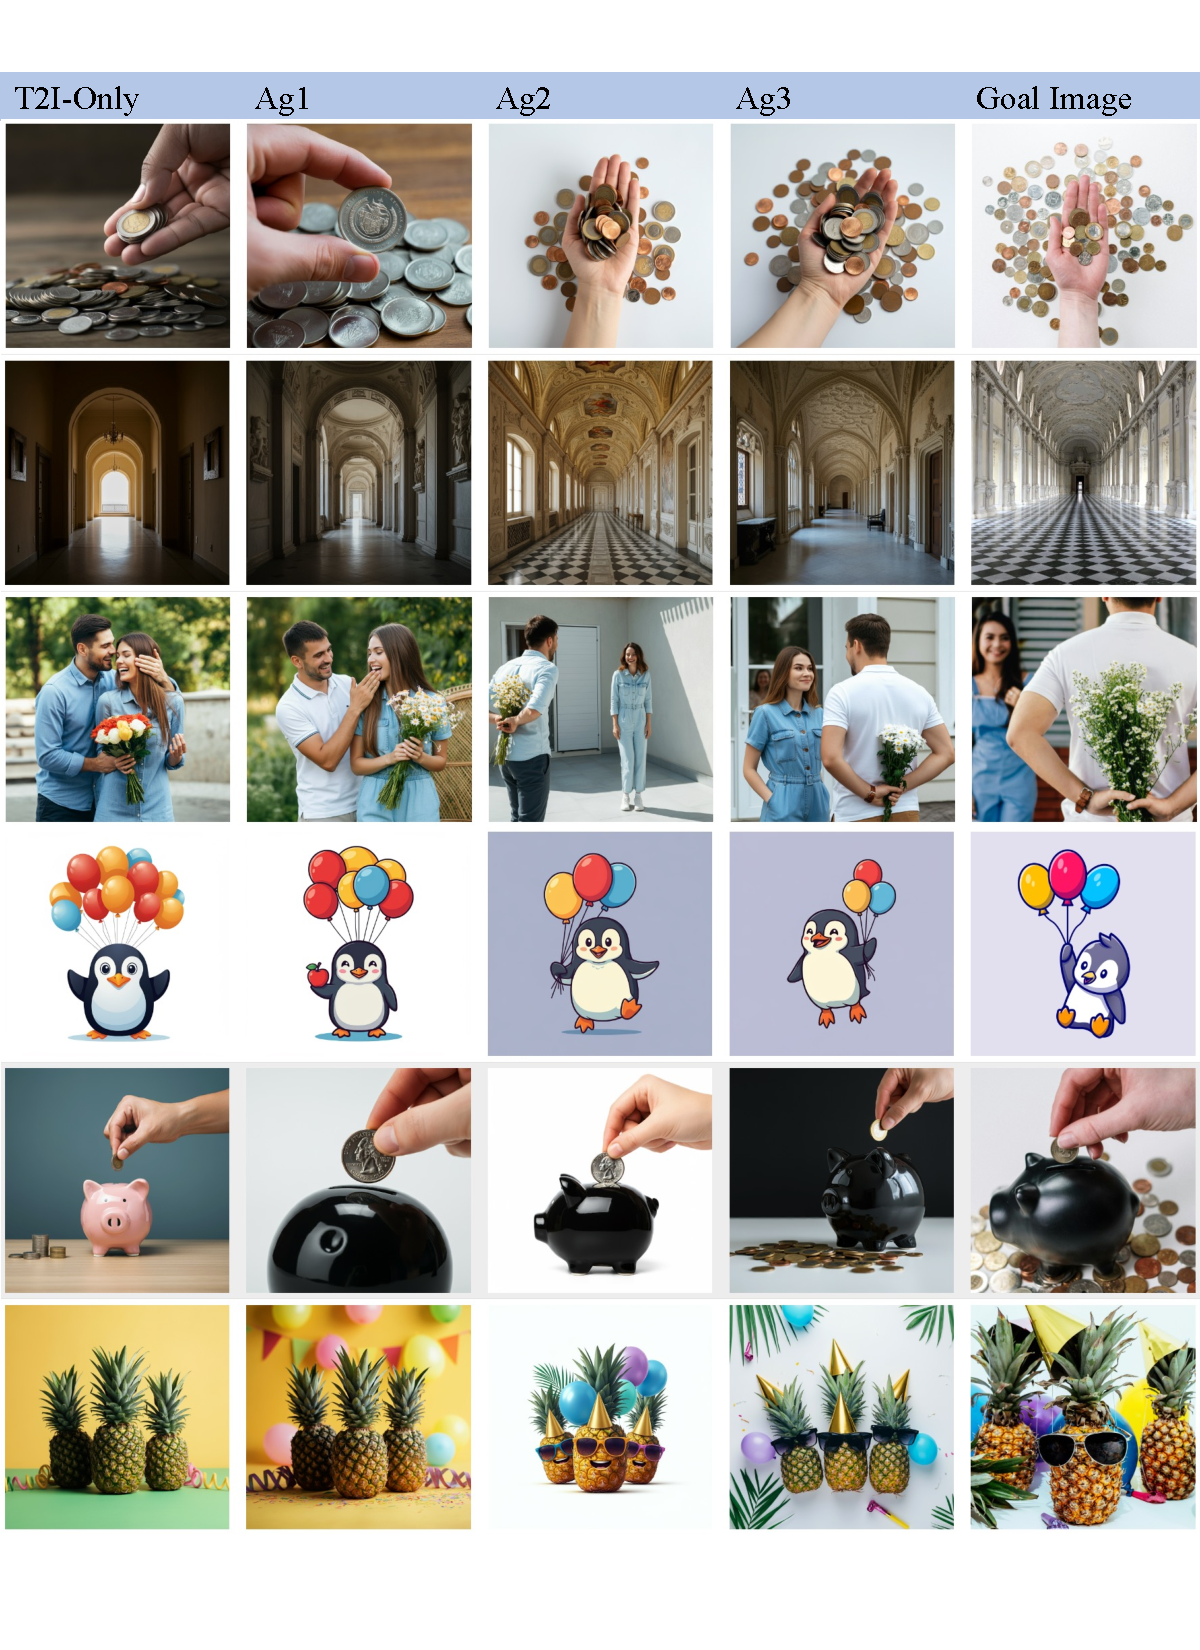
\includegraphics[width=\linewidth]{figures/toy_data_chart_part2.pdf}
    \caption{Agent Generated Image Outputs on DesignBench (Continued): a chart of the generated image outputs of the four main Agent types in comparison to the goal image. Each column displays the output of a different agent and the right most column shows the goal image that the agents aimed to recreate. Each agent was provided with the same starting prompt and iterated for 15 turns, with the exception of the "T2I" agent column which produces an image from the starting prompt. Ag1, Ag2 and Ag3 refer to the Agents described in \S \ref{ssec:implementation}. Each agent uses the same T2I model to produce the final image. The goal images displayed here are from the DesignBench dataset described in the experiments section.}
    \label{fig:toy2}
\end{figure}

\begin{figure}
    \centering
    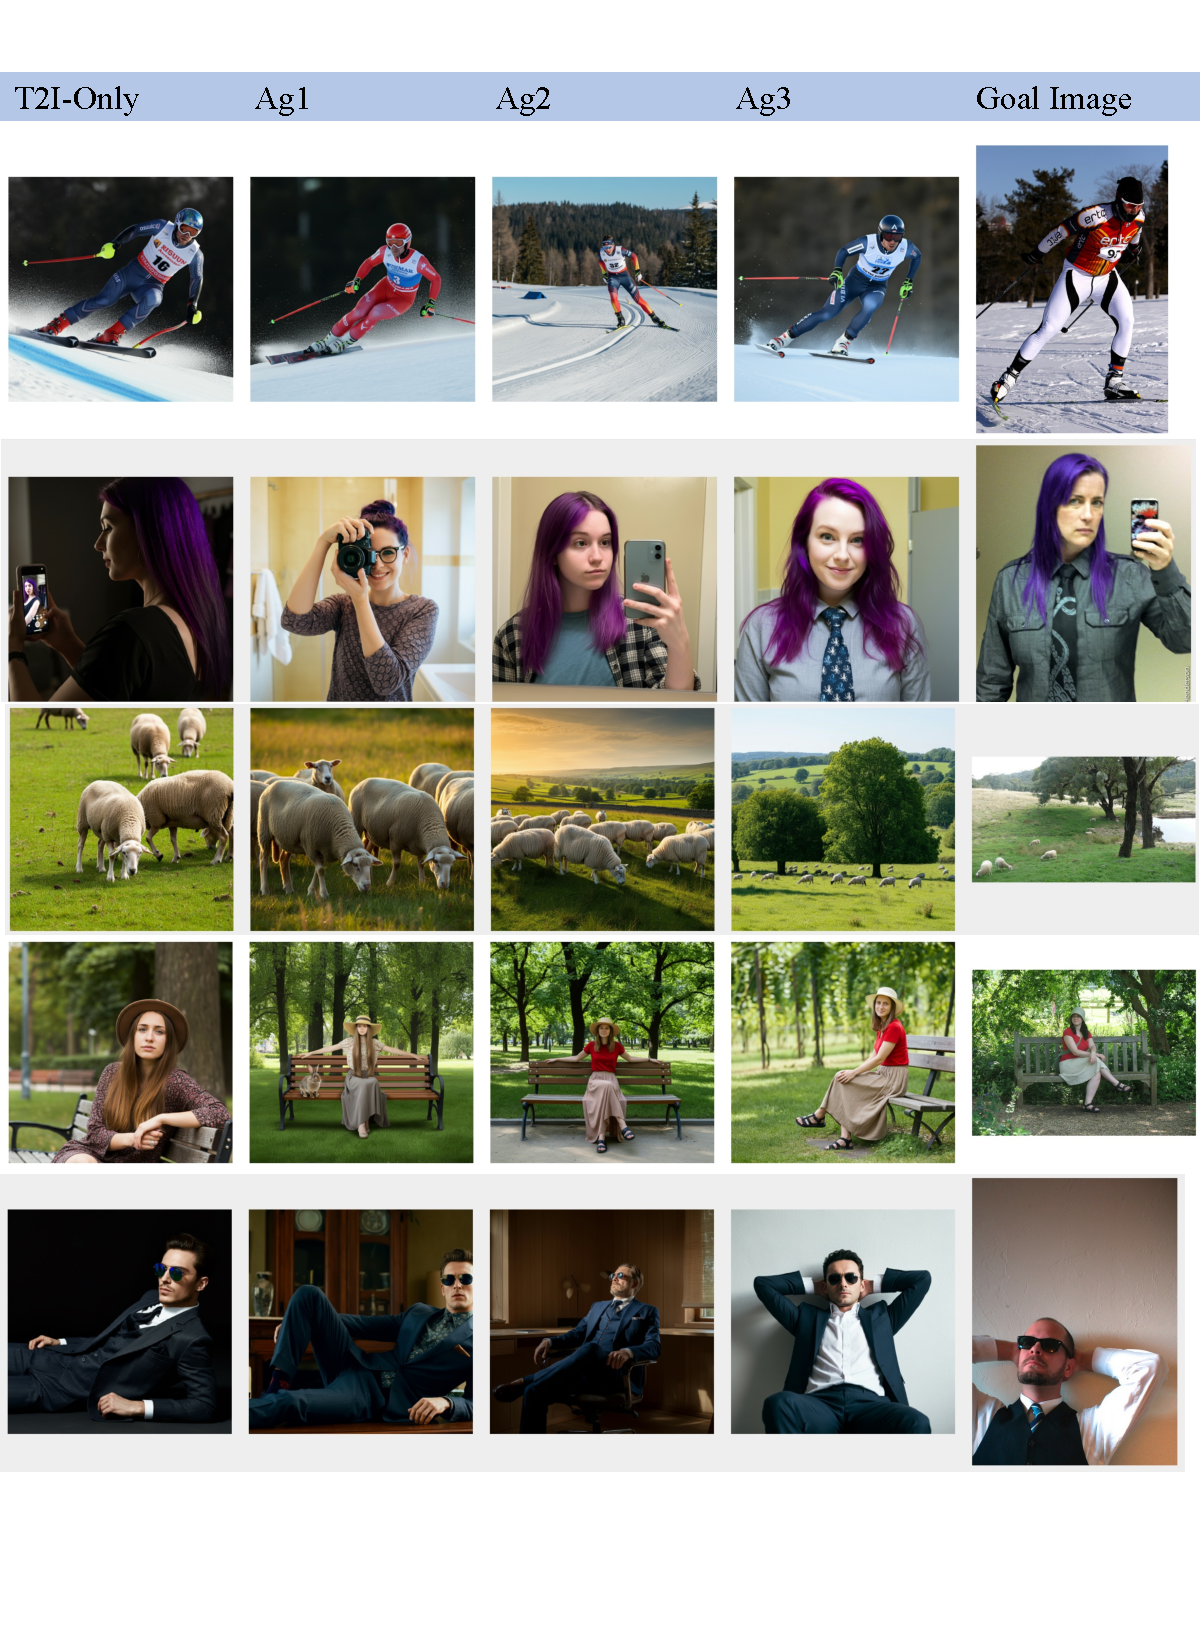
\includegraphics[width=\linewidth]{figures/coco_data_chart_part1.pdf}
    \caption{Agent Generated Image Outputs (Coco-Captions Validation): a chart of the generated image outputs of the four main Agent types in comparison to the goal image. Each column displays the output of a different agent and the right most column shows the goal image that the agents aimed to recreate. Each agent was provided with the same starting prompt and iterated for 15 turns, with the exception of the "T2I" agent column which produces an image from the starting prompt. Ag1, Ag2 and Ag3 refer to the Agents described in \S\ref{ssec:implementation}. Each agent uses the same T2I model to produce the final image. The goal images displayed here are from the Coco-Captions~\cite{chen2015microsoft} dataset described in the experiments section.}
    \label{fig:coco1}
\end{figure}

\begin{figure}
    \centering
    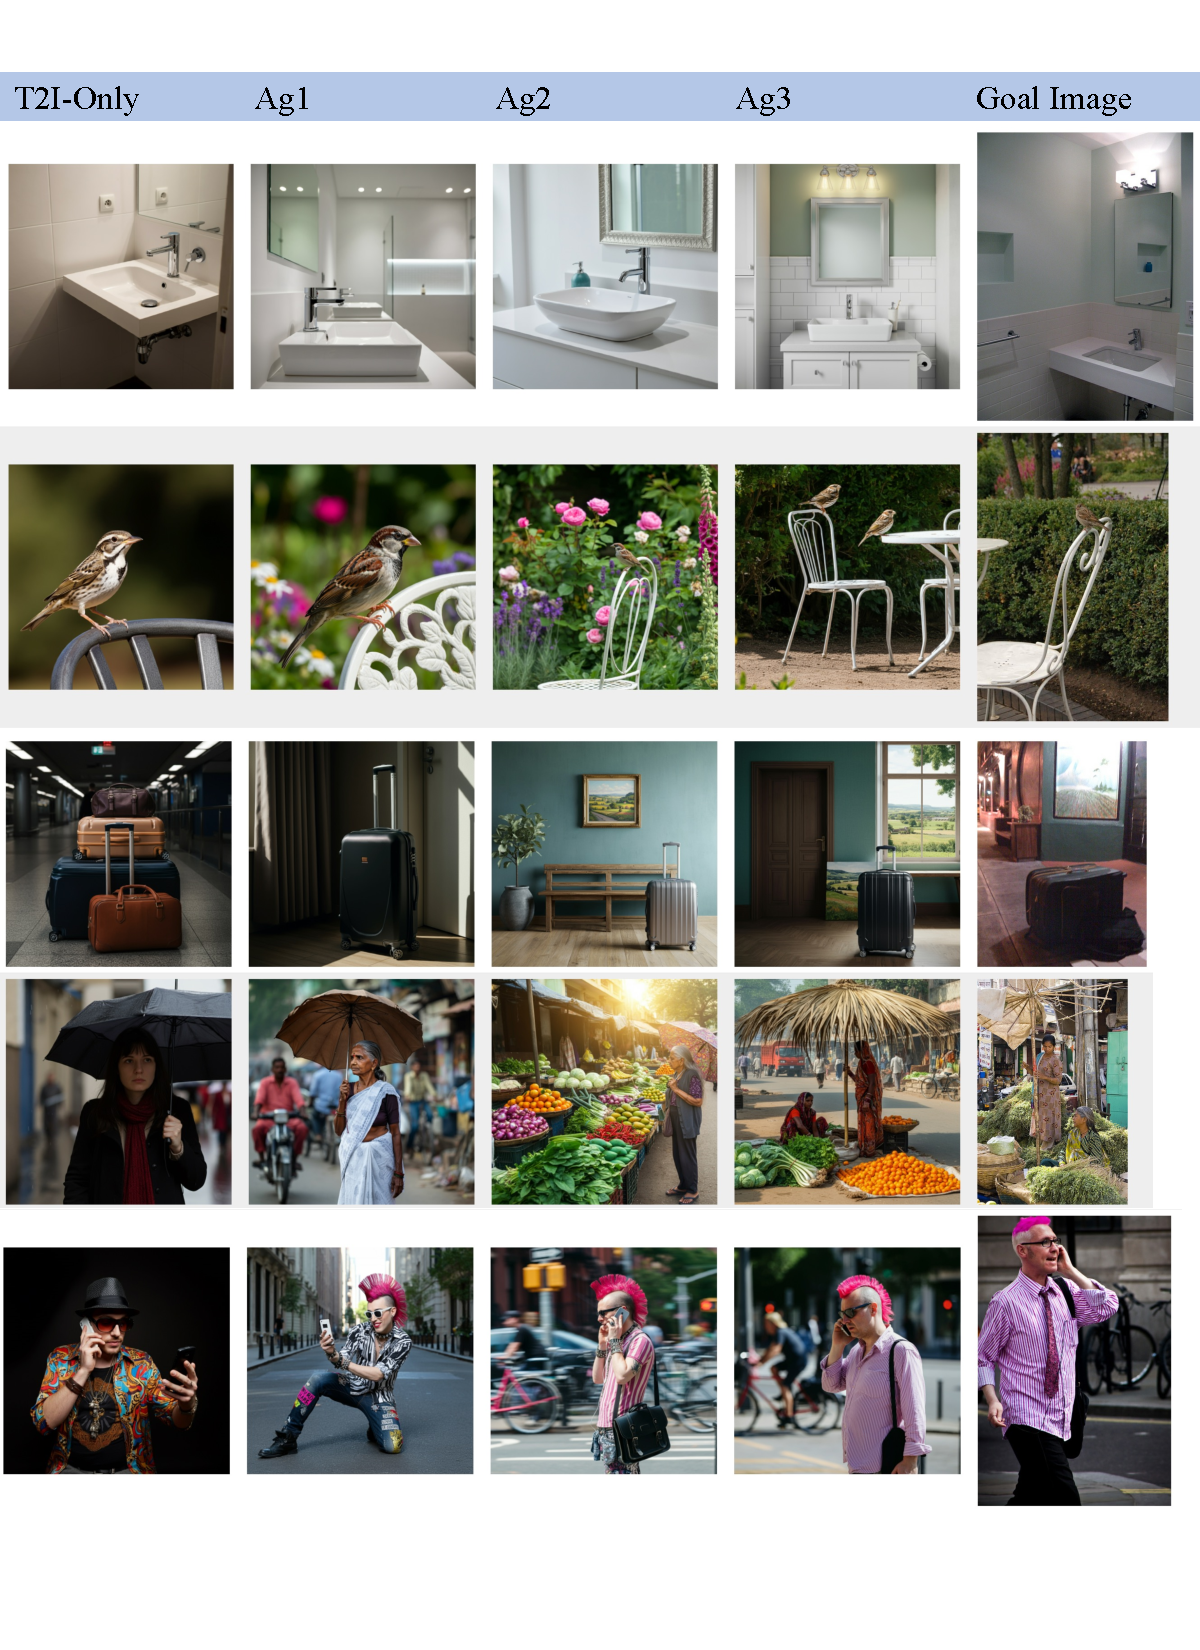
\includegraphics[width=\linewidth]{figures/coco_data_chart_part2.pdf}
    \caption{Agent Generated Image Outputs (Coco-Captions Validation): a chart of the generated image outputs of the four main Agent types in comparison to the goal image. Each column displays the output of a different agent and the right most column shows the goal image that the agents aimed to recreate. Each agent was provided with the same starting prompt and iterated for 15 turns, with the exception of the "T2I" agent column which produces an image from the starting prompt. Ag1, Ag2 and Ag3 refer to the Agent described in the methods section. Each agent uses the same T2I model to produce the final image. The goal images displayed here are from the Coco-Captions~\cite{chen2015microsoft} dataset described in the experiments section.}
    \label{fig:coco2}
\end{figure}
